\section{EppaBasic-ympäristö}
\fxnote{Kokoa tänne tavoitteet, käyttöliittymä ja kieli}

Tässä kappaleessa kerron EppaBasic-ympäristöstä
eli käyttöliittymästä ja ohjelmointikielestä.
Aluksi kuitenkin kerron ympäristölle
asettamistamme tavoitteista.

\subsection{Tavoitteet}
EppaBasicin tärkein tavoite on olla
mahdollisimman helppo oppia,
mutta samalla mahdollistaa
monipuolisten ohjelmien toteuttamisen.
Kielellä tytyy voida helposti luoda grafiikkaa,
sillä moni aloitteleva (ja miksei myös kokenutkin)
ohjelmoija haluaa nähdä työnsä tulokset.
Varsinkin aloittelijoille ohjelman aukeaminen
viime vuosituhannelta tuttuun komentokehotteen
(ks. Kuva \ref{img:cmd})
voi olla hyvinkin epätyydyttävää.
\fxnote{Media computation}

\begin{figure}[h]
    \centering
    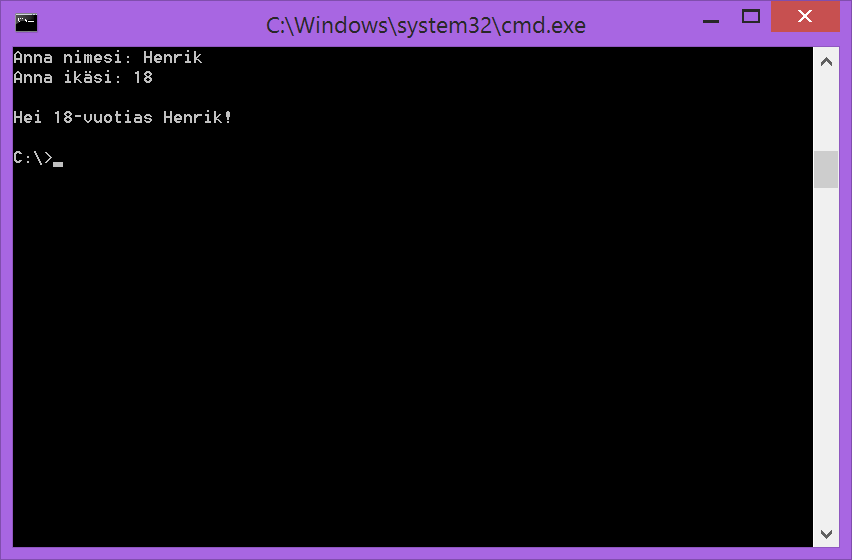
\includegraphics[width=1\textwidth]{cmd}
    \caption{Windowsin komentokehote yksinkertaisen python-ohjelman suorituksen jälkeen}
    \label{img:cmd}
\end{figure}

Toinen EppaBasicin tärkeä tavoite on olla
mahdollisimman helposti käyttöönotettava,
sillä usein uutta ohjelmointikieltä opetellessa
kuluu useita tunteja jo pelkän
ohjelmointiympäristön asentamiseen.
Tämän ajan voisi käyttää paljon tehokkaammin
itse kielen opettelemiseen.
\fxnote{Lannistavaa}

Ennen projektin aloittamista mietimme,
täyttäisikö jokin olemassa oleva kieli jo nämä tavoitteet.
Kuitenkin miettiessämme vaihtoehtoja
useat kielet olivat joko vanhentuneita,
niiden asentaminen tai oppiminen on hankalaa,
tai niillä grafiikan tekeminen on työlästä.
Tämän takia päädyimme uuden kielen tekemiseen.
Lisäksi ohjelmointikielten luominen on hauskaa
ja opettavaista.

\subsection{Käyttöliittymä}
EppaBasic-ympäristö koostuu kahdesta osasta,
joista ensimmäisenä esittelen ohjelmakoodin
kirjoittamiseen käytettävän käyttöliittymän.

\begin{figure}[h]
    \centering
    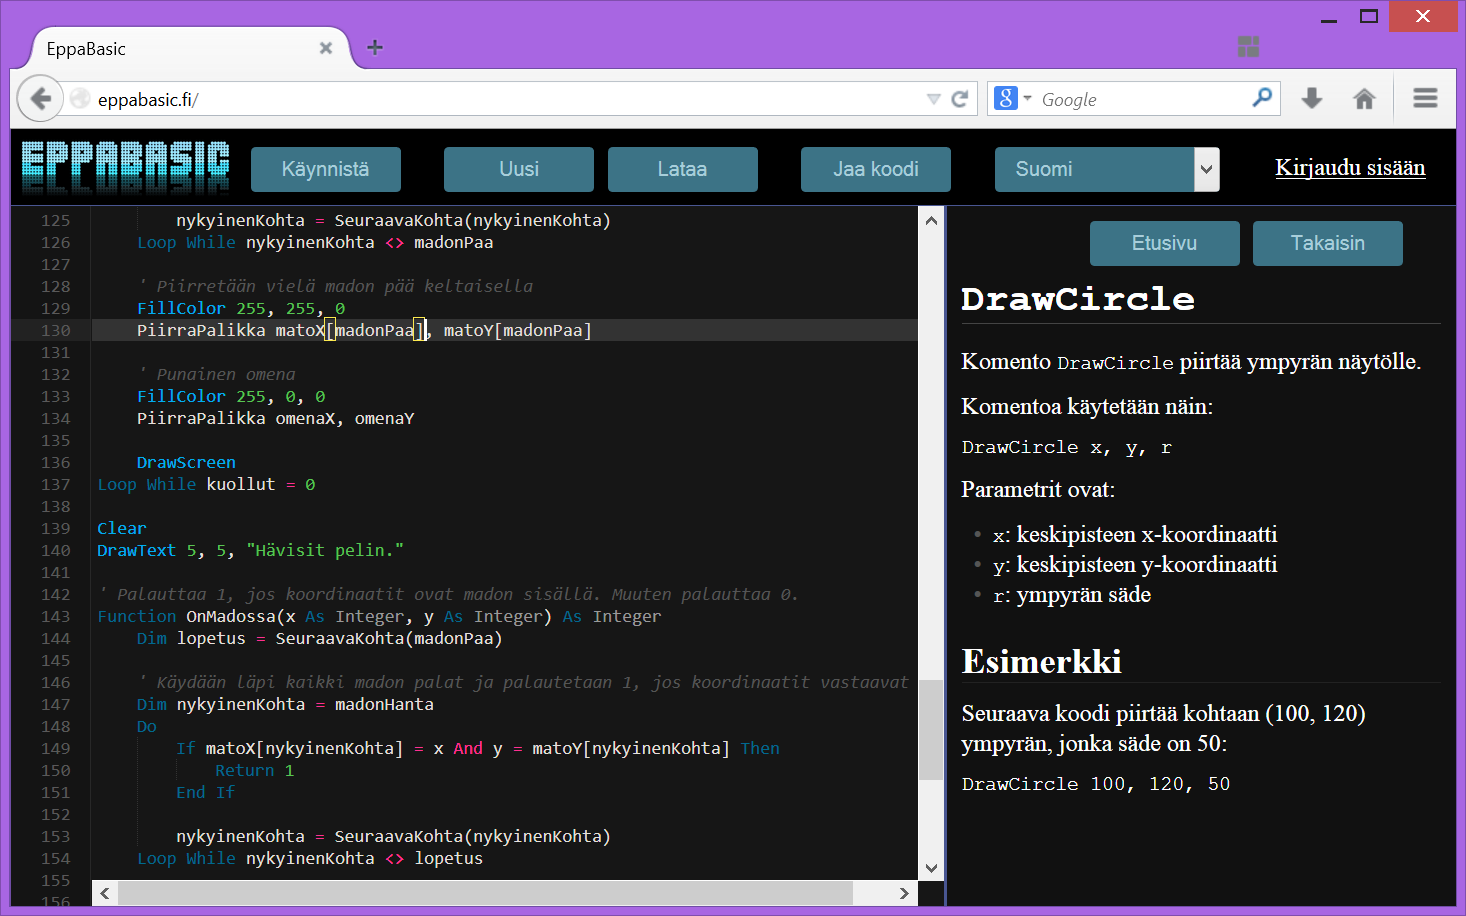
\includegraphics[width=1\textwidth]{kayttoliittyma}
    \caption{EppaBasicin käyttöiittymä}
    \label{img:kayttoliittyma}
\end{figure}

EppaBasicin käyttöliittymä on toteutettu
kokonaan käyttäen HTMLää ja JavaScriptiä.
Näin on saatu aikaan kaikissa moderneissa
selaimissa yhtenäinen käyttöliittymä.

EppaBasicin käyttöliittymä tarjoaa kaikki
ohjelmointiin tarvittavat toiminnot.
Yläpalkissa on koodin suorittamisen käynnistävä
nappi sekä napit koodin tallentamiseen ja lataamiseen.
Lisäksi koodin voi jakaa muille linkin avulla.
Kirjautumalla sisään koodin voi tallentaa
omalle käyttäjälleen, jolloin se on käytettävissä
kaikilla koneilla.

Käyttöliittymän vasemmalla reunalla on
suuri koodimuokkain, johon suoritettava
ohjelmakoodi kirjoitetaan.
Koodimuokkaimen oikealla puolella on
käyttöohje, jossa on kaikille
EppaBasicin tarjoamille funktioille
ja toiminnoille ohje esimerkkeineen.

EppaBasicin käyttämä tekstinmuokkain mahdollistaa
virheiden ilmoittamisen käyttäjälle jo hänen
kirjoittaessaan koodia.
Näin käyttäjä saa heti palautetta tekemistään
virheistä ja voi korjata ne samantien.
Jos käyttäjä ei huomaa virheen syytä,
hän voi lukea virheen sisältämän
kuvauksen virheestään omalla kielellään.

\subsection{Kieli}
EppaBasicin-ympäristön toinen osa on
itse ohjelmointikieli.
EppaBasic koostuu Basiceille tyypillisesti
englanninkielisistä avainsanista.
Komentrakenee koostuvat avainsanapareista,
joista parin ensimmäinen sana aloiaa komenorakenteen
ja toinen lopettaa sen.
Tällaisia pareja ovat esimerkiksi
$If$ ja $End If$,
$For$ ja $Next$
sekä $Do$ ja $Loop$.
Näin lopettavan avainsanan nähdessä on selvää,
minkä tyyppisen rakenteen se lopettaa,
tosin kuin esimerkiksi C-pohjaisissa
kielissä, joissa kaikki rakenteet alkavat
\{-merkillä ja loppuvat \}-merkkiin.
Myös rivinvaihdot ovat merkityksellisiä
Basic-kielissä, sillä jokainen lauseke
on kirjoitettava omalle rivilleen.


EppaBasic on vahvasti ja staattisesti tyypitetty.
Vahva tyypittäminen tarkoittaa sitä,
että tyypit muuttuvat vain erikoistapauksissa toisikseen
lausekkeita evaluoidessa.
Staattinen tyypittäminen tarkoittaa sitä,
että tietyn tyyppiseen muuttujaan voidaan tallentaa
vain muuttujan tyypin mukaisia arvoja.
Näin ei tule vahingossa tilanteita,
joissa muuttuja sisältääkin jotain muuta kuin pitäisi.
\fxnote{Ehkä jokin havainnollistus väärästä tyypistä,
kuten ''jossa lompakosta löytyykin kissa eikä rahaa''}